% Provenance (never printed): see sources/outline_sources.md (Year 1: physical and chemical
% weathering; hydrolysis and its degrees; the ionic-potential diagram; clay minerals and
% climate; silicate weathering and carbon dioxide). Exercise and problem values in the Book 3
% scratch calculator calc/ch19.py; figure data from figdata/bachelor-1/ionic_potential.py and
% hydrolysis.py. Weathering is owned by Book 1 g5; chemical weathering, hydrolysis, clay mineral
% and laterite by Book 2 g10 (re-founded here). Silicate classes and the feldspars by ch. 7;
% Bowen's series by Book 2 g11; acid--base chemistry, solubility and oxidation by the chemistry
% books; soils and their horizons by the biology books. The silicate-weathering thermostat
% belongs to the Year 2 volume (told).
\chapter{Meteorización y arcillas}\label{ch:b1:weathering-clays}

La inscripción de una antigua lápida se borra: los bordes afilados de las letras se redondean en surcos poco profundos, más deprisa
sobre un mármol que sobre una pizarra. Un afloramiento de granito que parece tan duro como cualquier cosa de la Tierra se desmorona en
su superficie hasta formar una arena áspera, que se escapa entre los dedos como granos sueltos de cuarzo vítreo, \omterm{def:b1:rock-forming-minerals:groups}{feldespato} terroso y
escamas de \omterm{def:b1:rock-forming-minerals:groups}{mica}. Bajo los bosques del trópico húmedo, la roca sólida puede yacer muy abajo, bajo una tierra roja que conserva los
contornos de los \omterm{def:b1:rock-forming-minerals:mineral}{minerales} de la roca pero se corta con una pala. Las tres cosas son obra del agua en la superficie de la Tierra. Este
capítulo escribe esa obra como química: qué \omterm{def:b1:rock-forming-minerals:mineral}{minerales} ceden primero, en qué se convierten, por qué algunos elementos salen con el agua
y otros se quedan, cómo fija el clima el resultado, y cómo la lenta descomposición de la roca silicatada extrae dióxido de carbono del aire.

\begin{recall}
La meteorización rompe las rocas en el lugar donde yacen (libro 1, año 5). La \omterm{def:b1:weathering-clays:weathering}{meteorización química} transforma los \omterm{def:b1:rock-forming-minerals:mineral}{minerales}; la
\omterm{def:b1:weathering-clays:hydrolysis}{hidrólisis} de un \omterm{def:b1:rock-forming-minerals:groups}{feldespato} da un \omterm{def:b1:rock-forming-minerals:mineral}{mineral} de arcilla, la \omterm{def:b1:weathering-clays:clay-mineral}{caolinita}, y envía potasio y sílice a los ríos; una \omterm{def:b1:weathering-clays:laterite}{laterita} es el producto rojo,
rico en hierro y aluminio, de los climas cálidos y húmedos (libro 2, año 10). Los silicatos se clasifican según cómo comparten las esquinas
sus tetraedros \ce{SiO4}: un \omterm{def:b1:rock-forming-minerals:silicate-classes}{filosilicato} forma láminas; los \omterm{def:b1:rock-forming-minerals:groups}{feldespatos} son silicatos de armazón de sodio, potasio y calcio, y las \omterm{def:b1:rock-forming-minerals:groups}{micas}
son \omterm{def:b1:rock-forming-minerals:silicate-classes}{filosilicatos} con potasio entre las láminas (\cref{def:b1:rock-forming-minerals:silicate-classes},
\cref{def:b1:rock-forming-minerals:groups}). El radio iónico de un ion depende de su carga y de su coordinación (\cref{ch:b1:rock-forming-minerals}).
Los \omterm{def:b1:rock-forming-minerals:mineral}{minerales} cristalizan de un magma en enfriamiento en el orden de la serie de reacciones de Bowen, primero el \omterm{def:b1:rock-forming-minerals:groups}{olivino} y último el
cuarzo (libro 2, año 11). Un ácido libera iones hidrógeno; el dióxido de carbono disuelto en agua forma ácido carbónico; una oxidación es
una pérdida de electrones; una ecuación ajustada conserva cada elemento y la carga (los libros de química). Un suelo es una capa viva
organizada en horizontes (los libros de biología).
\end{recall}

\section{Meteorización física y química}\label{sec:b1:weathering-clays:types}

Una roca formada en profundidad, a alta temperatura y presión y sin agua libre ni oxígeno, está fuera de equilibrio en la superficie.
Se ajusta de dos maneras, que actúan juntas.

\begin{definition}[Meteorización física, meteorización química]\label{def:b1:weathering-clays:weathering}
La \emph{meteorización física}\index{meteorización física} es la descomposición de una roca en su sitio en fragmentos más pequeños
sin cambio de sus \omterm{def:b1:rock-forming-minerals:mineral}{minerales}. La \emph{meteorización química}\index{meteorización química} es la transformación de los \omterm{def:b1:rock-forming-minerals:mineral}{minerales} de una roca
en su sitio por reacción con el agua y las sustancias que transporta, sobre todo iones hidrógeno, dióxido de carbono disuelto y oxígeno:
algunos \omterm{def:b1:rock-forming-minerals:mineral}{minerales} se disuelven, otros se sustituyen por \omterm{def:b1:rock-forming-minerals:mineral}{minerales} nuevos estables en la superficie, y parte de la roca sale en disolución.
\end{definition}
% ledger: formoso:weathering

\emph{Helada.} El agua a \qty{0}{\celsius} tiene la densidad
\qty{999.87}{kg.m^{-3}}, el hielo \qty{916.72}{kg.m^{-3}}: el agua se expande un
\qty{9.1}{\percent} al congelarse. La imagen antigua de la meteorización por helada es
el agua que se congela en una grieta cerrada y la fuerza a abrirse, de nuevo en cada
deshielo y congelación. Un modelo de grietas en granito y mármol, construido sobre la
mecánica de la fractura y sobre lo que se sabe de los suelos helados, pone el peso en otra parte: el agua es atraída a través de los
poros hacia el hielo ya presente en una grieta, como lo es hacia las lentes de hielo de un suelo helado, y el hielo crece y cuña la
grieta mientras dure la helada. La helada sostenida es más eficaz entre unos \qty{-4}{\celsius} y \qty{-15}{\celsius}: más cerca de
cero el hielo no puede acumular suficiente presión, y más frío el agua ya no puede desplazarse hacia él.
% ledger: usgs:water-density, iapws:ice-density, wh85:frost

\emph{Calentamiento, descarga y sal.} El calentamiento y el enfriamiento repetidos fatigan una roca cuyos \omterm{def:b1:rock-forming-minerals:mineral}{minerales} se dilatan en
cantidades distintas; un granito llevado a la superficie por la erosión, aliviado del peso que tenía encima, se expande y se parte en
láminas paralelas a la superficie; las sales que cristalizan del agua que se evapora, en los desiertos y las costas, separan los granos a palanca.

La \omterm{def:b1:weathering-clays:weathering}{meteorización física} hace más que romper la roca: la abre al agua.

\begin{proposition}[La superficie abierta por la fragmentación]\label{prop:b1:weathering-clays:surface}
Un cubo de lado $L$ cortado en cubos de lado $L/n$ tiene $n$ veces la superficie. De forma más general, una masa $m$ de granos de
densidad $\rho$, todos cubos de lado $d$, tiene la superficie $S = 6m/(\rho d)$: la superficie específica $S/m =
6/(\rho d)$ es inversamente proporcional al tamaño del grano.
\end{proposition}

\begin{proof}
Un cubo de lado $d$ tiene el área $6d^2$ y la masa $\rho d^3$, así que la superficie específica de cada grano, y de cualquier número de ellos, es $6d^2/(\rho d^3)
= 6/(\rho d)$. Cortar un cubo de lado $L$ en $n^3$ cubos de lado $L/n$ conserva la masa y divide $d$ entre $n$, lo que multiplica el área por $n$.
\end{proof}

Un bloque de \omterm{def:b1:rock-forming-minerals:groups}{feldespato} de densidad de unos \qty{2600}{kg.m^{-3}} tiene una superficie específica de \qty{0.23}{m^2.kg^{-1}} como fragmentos de
centímetro, y \qty{2.3}{m^2.g^{-1}} como granos de micrómetro, diez mil veces más. Las reacciones químicas proceden en las superficies, así que
una roca destrozada por la helada o abierta a lo largo de sus diaclasas se meteoriza químicamente mucho más deprisa que la misma roca intacta.
% ledger: hom:albite, hom:orthoclase

\emph{Las reacciones químicas.} La calcita se disuelve por completo en agua que lleva dióxido de carbono, por lo que las lápidas de mármol
pierden sus letras (libro 2, año 10). El hierro(II) de los silicatos oscuros se oxida a hierro(III), que queda en forma de óxidos amarillo-pardos
y rojos. Lo más importante, con mucho, porque los silicatos forman la mayor parte de la \omterm{def:b1:layered-earth:layers}{corteza}, es la \omterm{def:b1:weathering-clays:hydrolysis}{hidrólisis}. Los iones hidrógeno
proceden del dióxido de carbono, disuelto del aire y exhalado por las raíces y los descomponedores hacia el suelo, y de los ácidos
orgánicos de las plantas en descomposición: las aguas superficiales y del suelo no contaminadas tienen un pH entre 5.5 y 7, y el agua de
la capa orgánica de algunos suelos forestales llega a 3.5. El agua, la temperatura, la superficie y la acidez son así los cuatro controles
de la \omterm{def:b1:weathering-clays:weathering}{meteorización química}, y un clima cálido y húmedo con un suelo grueso proporciona los cuatro.
% ledger: formoso:weathering

\section{La hidrólisis de los silicatos}\label{sec:b1:weathering-clays:hydrolysis}

\begin{definition}[Hidrólisis de un silicato]\label{def:b1:weathering-clays:hydrolysis}
La \emph{hidrólisis}\index{hidrólisis (de silicatos)} de un silicato es su reacción con agua e iones hidrógeno en la que los iones
hidrógeno reemplazan a los cationes metálicos, que pasan a la disolución; parte o todo el silicio sale como ácido silícico disuelto
\ce{H4SiO4}, y el resto del \omterm{def:b1:rock-forming-minerals:mineral}{mineral} se reconstruye en un sólido nuevo, un \omterm{def:b1:rock-forming-minerals:mineral}{mineral} de arcilla o un hidróxido. La disolución es incongruente:
el sólido que queda no tiene la composición del \omterm{def:b1:rock-forming-minerals:mineral}{mineral} atacado.
\end{definition}
% ledger: formoso:weathering

El aluminio es la clave para escribir la reacción: al pH de los suelos y de los ríos es casi insoluble, y el producto sólido lo conserva todo.
Todo lo demás se deduce de eso.

\begin{method}[Ajuste de una reacción de hidrólisis]\label{met:b1:weathering-clays:balance}
Dados el \omterm{def:b1:rock-forming-minerals:mineral}{mineral} atacado y el producto sólido:
\begin{enumerate}
  \item Tómese una unidad formular del producto, y tanto del \omterm{def:b1:rock-forming-minerals:mineral}{mineral} como para que traiga el mismo número de átomos de aluminio.
  \item El silicio del \omterm{def:b1:rock-forming-minerals:mineral}{mineral} que no usa el producto sale como \ce{H4SiO4}; los cationes metálicos que no usa el producto salen como iones.
  \item Equilibrese la carga de estos cationes con iones hidrógeno a la izquierda.
  \item Equilibrese el oxígeno con agua a la izquierda.
  \item Compruébese el hidrógeno: debe equilibrarse por sí solo. Si no lo hace, una fórmula es errónea.
  \item Si se quiere una ecuación con coeficientes enteros, multiplíquese todo.
\end{enumerate}
\end{method}

\begin{proposition}[Hidrólisis de los feldespatos]\label{prop:b1:weathering-clays:feldspars}
Con la \omterm{def:b1:weathering-clays:clay-mineral}{esmectita} beidellita \ce{Na_{0.5}Al2(Si_{3.5}Al_{0.5})O10(OH)2}
(sin el agua interlaminar), la \omterm{def:b1:weathering-clays:clay-mineral}{caolinita} \ce{Al2Si2O5(OH)4} y la gibbsita
\ce{Al(OH)3} como productos,
\begin{align*}
&\ce{5 NaAlSi3O8 + 4 H+ + 16 H2O -> 2 Na_{0.5}Al2(Si_{3.5}Al_{0.5})O10(OH)2 + 4 Na+ + 8 H4SiO4},\\ % ce-unbalanced-ok: decimal subscripts the checker cannot read; balance tested in tests/bachelor-1/test_weathering_clays.py
&\ce{2 NaAlSi3O8 + 2 H+ + 9 H2O -> Al2Si2O5(OH)4 + 2 Na+ + 4 H4SiO4},\\
&\ce{NaAlSi3O8 + H+ + 7 H2O -> Al(OH)3 + Na+ + 3 H4SiO4},\\
&\ce{CaAl2Si2O8 + 2 H+ + H2O -> Al2Si2O5(OH)4 + Ca^2+}.
\end{align*}
La albita pierde el \qty{80}{\percent} de su sodio y $8/15$ de su silicio en la disolución en la primera reacción, todo su sodio y $2/3$ de su
silicio en la segunda, y todo lo de ambos en la tercera. La anortita pierde todo su calcio y ni un solo átomo de su silicio.
\end{proposition}
% ledger: webmineral:clays-b19, hom:albite, hom:anorthite

\begin{proof}
Aplíquese el método. Primera reacción: dos unidades de beidellita contienen $2\times2.5 = 5$ aluminios, el aluminio de 5 albitas; los 15
silicios de la albita menos los $2\times3.5 = 7$ del producto salen, quedando 8 \ce{H4SiO4}; los 5 sodios menos 1 quedan en 4 \ce{Na+}, equilibrados por
4 \ce{H+}; oxígeno, $40 + w$ a la izquierda y $24 + 32 =
56$ a la derecha, da $w = 16$; hidrógeno, $4 + 32 = 36$ y $4 + 32 = 36$, se comprueba. Segunda: 2 albitas dan los 2 aluminios de la \omterm{def:b1:weathering-clays:clay-mineral}{caolinita}, $6 - 2 = 4$
\ce{H4SiO4}, 2 \ce{Na+} y 2 \ce{H+}; oxígeno $16 + w = 9 + 16$ da $w = 9$; hidrógeno $2 + 18 = 20 = 4 + 16$. Tercera: una albita, tres ácidos silícicos, un
\ce{Na+} y un \ce{H+}; oxígeno $8 + w = 3 + 12$ da $w = 7$; hidrógeno $1 + 14 = 15 = 3 + 12$. Cuarta: los 2 aluminios y 2 silicios de la anortita son
exactamente los de la \omterm{def:b1:weathering-clays:clay-mineral}{caolinita}, no sale ningún ácido silícico, \ce{Ca^2+} necesita 2 \ce{H+}; oxígeno $8 + w = 9$ da $w = 1$; hidrógeno $2 + 2 = 4$. Las
fracciones exportadas son los iones en disolución sobre los átomos del \omterm{def:b1:rock-forming-minerals:mineral}{mineral}: $4/5$ y $8/15$, luego $2/2$ y $4/6$, luego $1/1$ y $3/3$.
\end{proof}

La misma albita puede dar, así, tres sólidos distintos, y cuál da depende de cuánta agua pase por la roca y se lleve los productos: poca agua, y
mucha de la sílice y algunos cationes se quedan para formar una \omterm{def:b1:weathering-clays:clay-mineral}{esmectita}; más agua, y solo queda la sílice suficiente para la \omterm{def:b1:weathering-clays:clay-mineral}{caolinita}; mucha
agua, y la sílice sale por completo.

\begin{definition}[Bisialitización, monosialitización, alitización]\label{def:b1:weathering-clays:hydrolysis-degree}
El grado de la \omterm{def:b1:weathering-clays:hydrolysis}{hidrólisis} de los silicatos se nombra por su producto.
La \emph{bisialitización}\index{bisialitización} forma \omterm{def:b1:rock-forming-minerals:mineral}{minerales} de arcilla 2:1, como las \omterm{def:b1:weathering-clays:clay-mineral}{esmectitas}, con unos dos átomos de silicio por
aluminio; parte de los cationes se queda en ellos. La \emph{monosialitización}\index{monosialitización} forma \omterm{def:b1:rock-forming-minerals:mineral}{minerales} de arcilla 1:1, la
\omterm{def:b1:weathering-clays:clay-mineral}{caolinita}, con un silicio por aluminio; salen todos los cationes alcalinos y alcalinotérreos. La \emph{alitización}\index{alitización} elimina
el silicio por completo y deja hidróxido de aluminio, la gibbsita.
\end{definition}
% ledger: pedron:stages, formoso:weathering

El grado alcanzado depende, ante todo, del clima, a través de la lluvia y la temperatura, y luego del drenaje del perfil. Donde el agua se renueva
poco, un granito pierde gran parte de su sodio y de su calcio, el potasio más despacio, y solo parte de su sílice: sus \omterm{def:b1:rock-forming-minerals:groups}{feldespatos} se convierten en
arcillas 2:1, y queda mucho cuarzo; la roca se desmorona en una arena de cuarzo, \omterm{def:b1:rock-forming-minerals:groups}{mica} y \omterm{def:b1:rock-forming-minerals:groups}{feldespato} a medio meteorizar mezclada con arcilla. Bajo las
lluvias intensas del trópico húmedo, más de \qty{2000}{mm} al año, los cationes y la sílice se lixivian mucho más, y se forma la \omterm{def:b1:weathering-clays:clay-mineral}{caolinita}, Si/Al = 1.
Donde la lixiviación es más intensa, incluso la sílice de la \omterm{def:b1:weathering-clays:clay-mineral}{caolinita} desaparece, y queda la gibbsita.
% ledger: pedron:stages, goldich:1938, formoso:laterite

\begin{omfigure}
\begin{tikzpicture}[font=\small]
% fractions of albite's Na and Si exported by the three degrees (figdata/bachelor-1/hydrolysis.py)
\begin{axis}[width=10.5cm, height=6cm, ybar, bar width=0.5cm, ymin=0, ymax=112,
    xmin=0.45, xmax=3.55, xtick={1,2,3},
    xticklabels={{bisialitización\\ hacia beidellita\\ (Si/Al = 1.4)}, {monosialitización\\ hacia caolinita\\ (Si/Al = 1)}, {alitización\\ hacia gibbsita\\ (Si/Al = 0)}},
    xticklabel style={align=center, font=\footnotesize},
    ylabel={exportado en disolución (\si{\percent})}, ytick={0,20,...,100},
    legend style={at={(0.5,1.03)}, anchor=south, font=\footnotesize, legend columns=2, draw=none},
    nodes near coords={\pgfmathprintnumber[fixed,precision=0]{\pgfplotspointmeta}}, every node near coord/.append style={font=\scriptsize},
    enlarge x limits=false]
  \addplot[fill=omThm!60, draw=omThm!80!black] table[x=degree, y=Na] {figdata/out/bachelor-1-hydrolysis-degrees.dat};
  \addplot[fill=omDef!55, draw=omDef!80!black] table[x=degree, y=Si] {figdata/out/bachelor-1-hydrolysis-degrees.dat};
  \legend{sodio, silicio}
\end{axis}
\end{tikzpicture}

{\small Los tres grados de \omterm{def:b1:weathering-clays:hydrolysis}{hidrólisis} de la albita: el porcentaje de su sodio y de su silicio que se lleva el agua en disolución, calculado a partir
de las reacciones ajustadas, y la razón silicio/aluminio del sólido que queda. El aluminio permanece por completo en el sólido en los tres.}
\label{fig:b1:weathering-clays:degrees}
\end{omfigure}


\begin{omfigure}
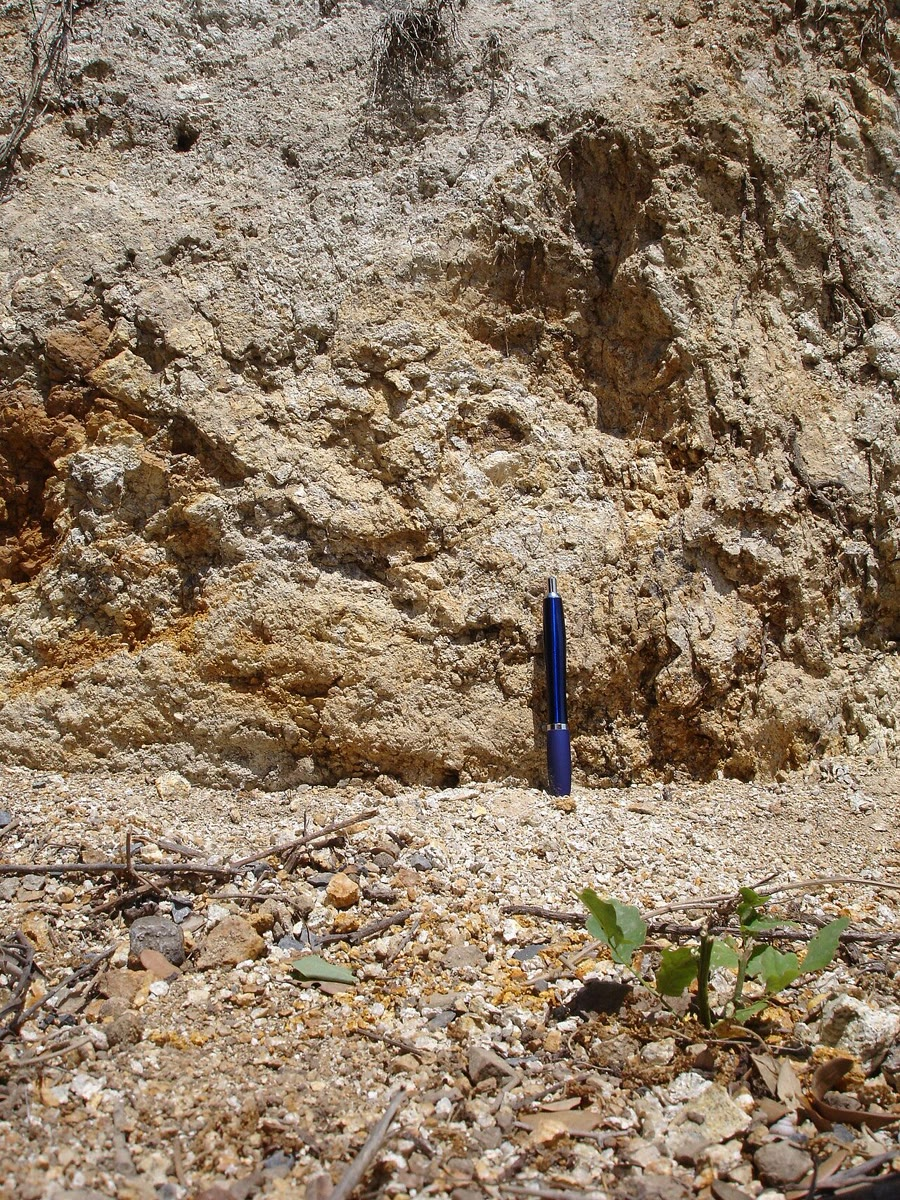
\includegraphics[height=6.3cm]{images/book3/b1-granite-grus.jpg}\hfill
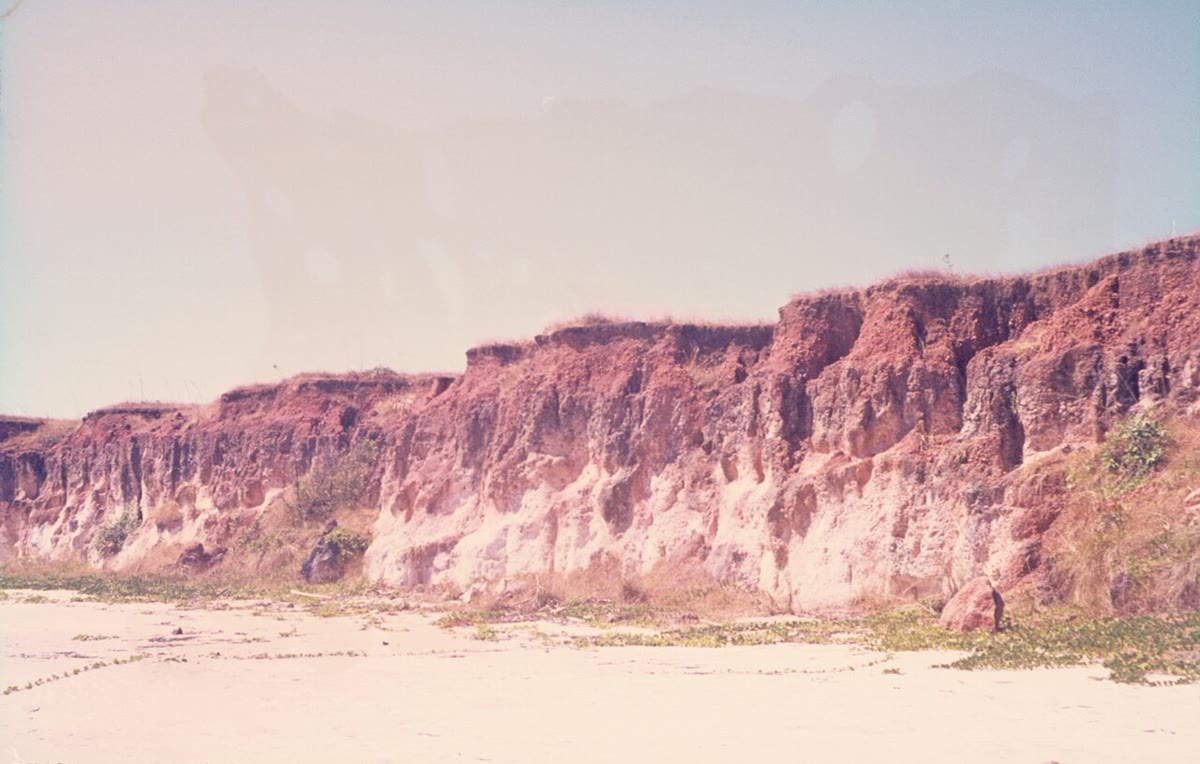
\includegraphics[height=6.3cm]{images/book3/b1-bauxite-weipa.jpg}
\par\smallskip{\small Izquierda: granito podrido en los Pirineos, todavía en su sitio pero desmoronándose en una arena de cuarzo, \omterm{def:b1:rock-forming-minerals:groups}{feldespato} y
\omterm{def:b1:rock-forming-minerals:groups}{mica}, con la arena suelta a su pie; el bolígrafo da la escala. Fotografía: Pinpin, CC~BY~2.5. Derecha: un perfil de meteorización en la
costa de Weipa, en el norte de Australia: bauxita roja, producto de la \omterm{def:b1:weathering-clays:hydrolysis-degree}{alitización}, sobre una arenisca blanca rica en \omterm{def:b1:weathering-clays:clay-mineral}{caolinita}. Fotografía:
Werner Schellmann, 1969, CC~BY-SA~2.5. Ambas de Wikimedia Commons.}
\label{fig:b1:weathering-clays:photos}
\end{omfigure}
% ledger: commons:grus, commons:weipa

\emph{Qué \omterm{def:b1:rock-forming-minerals:mineral}{minerales} se alteran primero.} En 1938 Samuel Goldich, comparando perfiles meteorizados con sus rocas madre, propuso una serie
de los \omterm{def:b1:rock-forming-minerals:mineral}{minerales} desde el menos hasta el más estable frente a la meteorización, y encontró que sigue el orden en que cristalizan de un
magma: primero el \omterm{def:b1:rock-forming-minerals:groups}{olivino} y el \omterm{def:b1:rock-forming-minerals:groups}{plagioclasa} rica en calcio, último el cuarzo. Los \omterm{def:b1:rock-forming-minerals:mineral}{minerales} formados a las temperaturas más altas son los más
alejados del equilibrio en la superficie. Una lista moderna, de menos a más resistente, dice: pirita, calcita, dolomita, \omterm{def:b1:rock-forming-minerals:groups}{olivino}, \omterm{def:b1:rock-forming-minerals:groups}{plagioclasa}
cálcica, \omterm{def:b1:rock-forming-minerals:groups}{piroxenos}, \omterm{def:b1:rock-forming-minerals:groups}{plagioclasa} intermedia, \omterm{def:b1:rock-forming-minerals:groups}{anfíboles}, biotita, \omterm{def:b1:rock-forming-minerals:groups}{feldespato} potásico, moscovita, \omterm{def:b1:weathering-clays:clay-mineral}{esmectita}, cuarzo, \omterm{def:b1:weathering-clays:clay-mineral}{caolinita}, y los óxidos
gibbsita y hematites. Las medidas de laboratorio de las velocidades de disolución confirman la clasificación; sigue siendo una clasificación,
no una ley, pues la velocidad de cada \omterm{def:b1:rock-forming-minerals:mineral}{mineral} depende también del agua que lo rodea. Los productos finales de la meteorización, \omterm{def:b1:weathering-clays:clay-mineral}{caolinita},
gibbsita y hematites, son los más resistentes de todos: ya son estables en la superficie.
% ledger: goldich:1938, formoso:weatherability, lasaga:1984

\emph{El balance de un perfil de meteorización.} La meteorización elimina materia, así que una concentración medida en una roca meteorizada no
dice cuánto se perdió: la pérdida de otros elementos concentra los que permanecen. Un elemento que no se mueve da la referencia.

\begin{proposition}[Balance de masa con un elemento inmóvil]\label{prop:b1:weathering-clays:immobile}
Sea $i$ un elemento que la meteorización no mueve, con fracciones másicas
$C_{i,p}$ en la roca madre y $C_{i,w}$ en la roca meteorizada. Entonces una masa
$m_p$ de roca madre se convierte en la masa $m_w = m_p C_{i,p}/C_{i,w}$ de roca
meteorizada, y la fracción de cualquier otro elemento $j$ perdida es
\[
  f_j = 1 - \frac{C_{j,w}}{C_{j,p}}\,\frac{C_{i,p}}{C_{i,w}} .
\]
\end{proposition}

\begin{proof}
La masa de $i$ se conserva: $m_p C_{i,p} = m_w C_{i,w}$, lo que da $m_w$.
La masa de $j$ pasa de $m_p C_{j,p}$ a $m_w C_{j,w}$, quedando una fracción
$m_w C_{j,w}/(m_p C_{j,p}) = (C_{j,w}/C_{j,p})(C_{i,p}/C_{i,w})$ de ella; $f_j$ es uno menos esta fracción.
\end{proof}

El titanio y el circonio son las elecciones habituales, por una razón que da la sección siguiente.

\section{Qué elementos salen: el potencial iónico}\label{sec:b1:weathering-clays:ionic}

El sodio, el potasio y el calcio salen con el agua; el aluminio, el hierro(III) y el titanio permanecen; el silicio está en medio. La diferencia
está en cómo se comporta cada ion en el agua.

\begin{definition}[Potencial iónico]\label{def:b1:weathering-clays:ionic-potential}
El \emph{potencial iónico}\index{potencial iónico} de un ion es el cociente $z/r$
de su número de carga $z$ entre su radio iónico $r$, aquí en ångströms (para la misma coordinación para todos los iones, la sexta en lo que sigue).
\end{definition}
% ledger: nomad:goldschmidt, dangic:goldschmidt, shannon:radii-b19

\begin{proposition}[Los tres campos del potencial iónico]\label{prop:b1:weathering-clays:fields}
En el agua de la meteorización, los iones con $z/r < 3$ permanecen en disolución como cationes hidratados y son arrastrados (cationes solubles);
los iones con $3 < z/r < 10$ fijan los iones hidróxido del agua y precipitan como hidróxidos u óxidos allí donde se liberan (hidrolizados);
los iones con $z/r > 10$ fijan tan fuertemente el oxígeno que repelen los iones hidrógeno y viajan como oxianiones solubles, como el carbonato,
el sulfato, el fosfato y el nitrato. El silicio, con $z/r = 10$, queda en el límite, y se lixivia en parte, tanto más cuanto más intensa es la meteorización.
\end{proposition}
\admitted
% ledger: nomad:goldschmidt, dangic:goldschmidt

La regla es empírica, debida a Victor Moritz Goldschmidt en los años treinta, y sus límites son aproximados; la química que hay detrás, la atracción
entre un catión y el oxígeno de las moléculas de agua que lo rodean, pertenece a los libros de química. Un catión pequeño y muy cargado tira de los
electrones de sus moléculas de agua con tanta fuerza que estas pierden un ion hidrógeno y se convierten en hidróxido: con moderación, y el hidróxido
precipita; con extremo, y hasta el hidróxido pierde su hidrógeno, dejando un oxianión.

El diagrama de abajo permite leer de un vistazo la meteorización de una roca. El sodio ($z/r = 0.98$), el potasio (0.72), el calcio (2.0) y el
magnesio (2.8) salen: son los cationes del agua de los ríos y del mar. El aluminio (5.6), el hierro(III) (4.7), el titanio (6.6) y el circonio (5.6)
permanecen, y se acumulan en los perfiles más meteorizados; el titanio y el circonio, que además están en \omterm{def:b1:rock-forming-minerals:mineral}{minerales} que apenas se meteorizan, son las
referencias inmóviles de \cref{prop:b1:weathering-clays:immobile}. El silicio (10.0) es el elemento cuya pérdida parcial define los grados de la \omterm{def:b1:weathering-clays:hydrolysis}{hidrólisis}.
% ledger: shannon:radii-b19

La oxidación desplaza un ion a través del límite. El hierro(II), con $z/r = 2.6$, es un catión soluble; el hierro(III), con 4.7, un hidrolizado. En un
suelo encharcado y sin oxígeno, el hierro se disuelve como \ce{Fe^2+} y es arrastrado, dejando un suelo gris; donde el agua encuentra el aire, en un
manantial o en un suelo bien drenado, el hierro se oxida y precipita de inmediato como óxidos rojos y pardos. El manganeso se comporta igual,
\ce{Mn^2+} (2.4) frente a \ce{Mn^4+} (7.5).
% ledger: nomad:goldschmidt, shannon:radii-b19

\begin{omfigure}
\begin{tikzpicture}[font=\small]
% ionic-potential diagram (figdata/bachelor-1/ionic_potential.py): charge against Shannon radius
\begin{axis}[width=12.5cm, height=8.4cm, xmin=0, xmax=1.8, ymin=0, ymax=7,
    xlabel={radio iónico $r$ (\si{\angstrom}, coordinación sexta)}, ylabel={carga $z$},
    ytick={1,...,6}, xtick={0,0.2,...,1.8}, xticklabel style={/pgf/number format/fixed},
    axis on top, clip=true]
  \fill[omThm!14] (axis cs:0,0) -- (axis cs:1.8,0) -- (axis cs:1.8,5.4) -- cycle;
  \fill[omDef!16] (axis cs:0,0) -- (axis cs:1.8,5.4) -- (axis cs:1.8,7) -- (axis cs:0.7,7) -- cycle;
  \fill[omExo!18] (axis cs:0,0) -- (axis cs:0.7,7) -- (axis cs:0,7) -- cycle;
  \addplot[black, thick] table[x=r, y=z3] {figdata/out/bachelor-1-ionic_potential-lines.dat};
  \addplot[black, thick] table[x=r, y=z10] {figdata/out/bachelor-1-ionic_potential-lines.dat};
  \addplot[only marks, mark=*, mark size=1.6pt, black,
      point meta=explicit symbolic, nodes near coords,
      visualization depends on={value \thisrow{anc} \as \anc},
      every node near coord/.append style={font=\scriptsize, inner sep=2.6pt, anchor=\anc}]
    table[x=r, y=z, meta=tex] {figdata/out/bachelor-1-ionic_potential-ions.dat};
  \node[font=\footnotesize, align=center, fill=white, fill opacity=0.8, text opacity=1, rounded corners=1pt] at (axis cs:1.45,2.75) {cationes solubles\\ $z/r < 3$};
  \node[font=\footnotesize, align=center, fill=white, fill opacity=0.8, text opacity=1, rounded corners=1pt] at (axis cs:1.15,6.3) {hidrolizados\\ $3 < z/r < 10$};
  \node[font=\footnotesize, align=left, fill=white, fill opacity=0.8, text opacity=1, rounded corners=1pt, anchor=north west] at (axis cs:0.015,6.95) {oxianiones solubles, $z/r > 10$};
  \node[font=\scriptsize, rotate=28, anchor=south] at (axis cs:1.62,4.86) {$z/r = 3$};
  \node[font=\scriptsize, rotate=61, anchor=south] at (axis cs:0.2,2.0) {$z/r = 10$};
\end{axis}
\end{tikzpicture}

{\small El diagrama del \omterm{def:b1:weathering-clays:ionic-potential}{potencial iónico}: cada ion situado por su radio iónico efectivo en coordinación sexta (Shannon, 1976) y su carga.
Las rectas $z/r = 3$ y $z/r = 10$ separan los iones que salen en disolución como cationes, los que quedan como hidróxidos u óxidos, y los que salen
como oxianiones. El silicio queda sobre el límite superior.}
\label{fig:b1:weathering-clays:ionic-potential}
\end{omfigure}
% ledger: shannon:radii-b19, nomad:goldschmidt

\section{Minerales de la arcilla}\label{sec:b1:weathering-clays:clays}

\begin{definition}[Mineral de la arcilla, caolinita, ilita, esmectita, clorita]\label{def:b1:weathering-clays:clay-mineral}
Un \emph{mineral de la arcilla}\index{mineral de la arcilla} es un \omterm{def:b1:rock-forming-minerals:silicate-classes}{filosilicato} de aluminio hidratado, por lo común en granos de unos pocos micrómetros
o menos, formado por capas que combinan una lámina tetraédrica (T) de tetraedros \ce{SiO4} que comparten tres esquinas y una lámina octaédrica (O)
de aluminio o magnesio rodeada de oxígeno e hidroxilo. En la \emph{caolinita}\index{caolinita}, \ce{Al2Si2O5(OH)4}, cada capa es una lámina T y una lámina O
(una capa 1:1 o T--O), sin carga, y las capas se mantienen unidas por enlaces de hidrógeno. En los \omterm{def:b1:rock-forming-minerals:mineral}{minerales} de arcilla 2:1 o T--O--T una lámina O yace
entre dos láminas T que apuntan hacia ella: la \emph{ilita}\index{ilita} es un \omterm{def:b1:rock-forming-minerals:mineral}{mineral} de arcilla 2:1 no expansible con iones potasio entre las capas, como una \omterm{def:b1:rock-forming-minerals:groups}{mica} con
menos potasio; una \emph{esmectita}\index{esmectita} es un \omterm{def:b1:rock-forming-minerals:mineral}{mineral} de arcilla 2:1 con cationes hidratados e intercambiables y agua entre sus capas, que puede
absorber más agua e hincharse; una \emph{clorita}\index{clorita} es un \omterm{def:b1:rock-forming-minerals:mineral}{mineral} 2:1 cuyas capas cargadas negativamente se alternan con láminas octaédricas
cargadas positivamente de tipo brucita, \ce{(Mg,Fe)(OH)2} con algo de aluminio.
\end{definition}
% ledger: usgs:clay-groups, usgs:clay-settings, webmineral:clays-b19, biscaye:1965

La carga de una capa decide cómo se apilan las capas, y la carga procede de las sustituciones en las láminas (\cref{def:b1:rock-forming-minerals:substitution}).

\begin{proposition}[Carga de una capa 2:1]\label{prop:b1:weathering-clays:layer-charge}
Una capa 2:1 de fórmula $\mathrm{(Si_{4-x}Al_x)(Al_{2-y}Mg_y)O_{10}(OH)_2}$, con
$x$ aluminios por silicio en sus láminas tetraédricas e $y$ magnesios por
aluminio en su lámina octaédrica, lleva la carga $-(x + y)$ por unidad formular.
\end{proposition}

\begin{proof}
Súmense las cargas: $4(4 - x) + 3x$ de los cationes tetraédricos, $3(2 - y) + 2y$
de los octaédricos, $-2\times10$ de los oxígenos y $-1\times2$ de los hidroxilos: $16 - x + 6 - y - 20 - 2 = -(x + y)$.
\end{proof}

Sin sustitución ($x = y = 0$) la capa es neutra, como en \ce{Al2Si4O10(OH)2}, el \omterm{def:b1:rock-forming-minerals:mineral}{mineral} pirofilita, y las capas se mantienen unidas solo por fuerzas
débiles. En la moscovita, $x = 1$; una carga de $-1$ se equilibra con un ion potasio que une las capas; la \omterm{def:b1:weathering-clays:clay-mineral}{ilita} está cerca de ella, con algo menos.
En la beidellita de \cref{prop:b1:weathering-clays:feldspars}, $x = 0.5$: la carga $-0.5$ se equilibra con $0.5$ sodio. Una carga menor sujeta las capas
con menos fuerza, y entre ellas pueden entrar agua y cationes hidratados: por eso las \omterm{def:b1:weathering-clays:clay-mineral}{esmectitas}, con cargas de unos 0.3 a 0.5 por unidad formular, como
en las fórmulas de la montmorillonita y de la beidellita, se hinchan, mientras que la \omterm{def:b1:weathering-clays:clay-mineral}{ilita} no lo hace. Los cationes entre las capas de una \omterm{def:b1:weathering-clays:clay-mineral}{esmectita} son
intercambiables, y la capacidad de intercambio de los \omterm{def:b1:rock-forming-minerals:mineral}{minerales} de arcilla comunes sigue a su estructura: 3 a 15 miliequivalentes por
\qty{100}{g} en la \omterm{def:b1:weathering-clays:clay-mineral}{caolinita}, cuyas capas no tienen carga; de 10 a 40 para la \omterm{def:b1:weathering-clays:clay-mineral}{ilita}; de 70 a 100 para la montmorillonita, una \omterm{def:b1:weathering-clays:clay-mineral}{esmectita}.
El potasio, que une las capas de una \omterm{def:b1:rock-forming-minerals:groups}{mica}, favorece la \omterm{def:b1:weathering-clays:clay-mineral}{ilita}; las \omterm{def:b1:weathering-clays:clay-mineral}{esmectitas} se forman donde escasea el potasio y hay calcio y magnesio disponibles.
% ledger: webmineral:clays-b19, carroll:cec, usgs:clay-settings

\begin{omfigure}
\begin{tikzpicture}[font=\footnotesize, >={Stealth[length=4pt]}, y=0.2cm, x=1cm]
% schematic clay-mineral structures, vertical scale proportional to the basal spacings
% (USGS OFR 01-041, ledger usgs:clay-xrd): kaolinite 7, illite 10, smectite 14 (air-dried), chlorite 14 angstrom.
% T sheet 2 A thick, O sheet 2.4 A thick (schematic); the column width is 2.2 cm.
\def\W{2.2}
\newcommand{\Tsheet}[1]{% tetrahedral sheet whose base is at y=#1
  \fill[omDef!35] (0,#1) rectangle (\W,#1+2);
  \foreach \i in {0,...,6} {\draw[omDef!80!black, line width=0.4pt] (0.04+\i*0.31,#1) -- (0.195+\i*0.31,#1+2) -- (0.35+\i*0.31,#1) -- cycle;}
}
\newcommand{\TsheetDown}[1]{% inverted tetrahedral sheet, base at the top (y=#1+2)
  \fill[omDef!35] (0,#1) rectangle (\W,#1+2);
  \foreach \i in {0,...,6} {\draw[omDef!80!black, line width=0.4pt] (0.04+\i*0.31,#1+2) -- (0.195+\i*0.31,#1) -- (0.35+\i*0.31,#1+2) -- cycle;}
}
\newcommand{\Osheet}[2]{% octahedral sheet, base at y=#1, fill colour #2
  \fill[#2] (0,#1) rectangle (\W,#1+2.4);
  \foreach \i in {0,...,4} {\draw[black!55, line width=0.4pt] (0.17+\i*0.42,#1+1.2) -- ++(0.17,1.0) -- ++(0.17,-1.0) -- ++(-0.17,-1.0) -- cycle;}
}
\newcommand{\spacing}[3]{% arrow for d001 from y=#1 to y=#2 with label #3
  \draw[<->, line width=0.5pt] (\W+0.18,#1) -- (\W+0.18,#2) node[midway, right, inner sep=2pt] {#3};
  \draw[black!40, densely dotted] (\W,#1) -- (\W+0.28,#1); \draw[black!40, densely dotted] (\W,#2) -- (\W+0.28,#2);
}
% ---------- kaolinite: T-O, d = 7.2
\begin{scope}[xshift=0cm]
  \foreach \b in {0, 7.2} {\Tsheet{\b} \Osheet{\b+2}{omThm!25}}
  \spacing{0}{7.2}{\SI{7}{\angstrom}}
\node[anchor=north, align=center] at (\W/2,-0.8) {\textbf{caolinita}\\ capas T--O (1:1)\\ unidas por enlaces de hidrógeno};
\end{scope}
% ---------- illite: T-O-T + K, d = 10
\begin{scope}[xshift=3.6cm]
  \foreach \b in {0, 10} {\Tsheet{\b} \Osheet{\b+2}{omThm!25} \TsheetDown{\b+4.4}}
  \foreach \b in {6.4} {\foreach \i in {0,...,4} \fill[omExo!70!black] (0.25+\i*0.42,\b+1.8) circle[radius=1.5pt];}
  \spacing{0}{10}{\SI{10}{\angstrom}}
  \node[anchor=north, align=center] at (\W/2,-0.8) {\textbf{ilita}\\ capas T--O--T (2:1)\\ unidas por iones \ce{K+}};
\end{scope}
% ---------- smectite: T-O-T + hydrated cations, d = 14
\begin{scope}[xshift=7.2cm]
  \foreach \b in {0, 14} {\Tsheet{\b} \Osheet{\b+2}{omThm!25} \TsheetDown{\b+4.4}}
  \foreach \i in {0,...,9} {\draw[omDef!60, line width=0.3pt] (0.13+\i*0.215,8.6) circle[radius=1.3pt]; \draw[omDef!60, line width=0.3pt] (0.2+\i*0.215,11.8) circle[radius=1.3pt];}
  \foreach \i in {0,...,3} {\fill[omExo!70!black] (0.35+\i*0.5,10.2) circle[radius=1.5pt];}
  \spacing{0}{14}{\SI{14}{\angstrom}}
  \node[anchor=north, align=center] at (\W/2,-0.8) {\textbf{esmectita}\\ capas T--O--T, hidratadas\\ con \ce{Na+}, \ce{Ca^2+} y agua};
\end{scope}
% ---------- chlorite: T-O-T + brucite-like O sheet, d = 14
\begin{scope}[xshift=10.8cm]
  \foreach \b in {0, 14} {\Tsheet{\b} \Osheet{\b+2}{omThm!25} \TsheetDown{\b+4.4}}
  \Osheet{9}{omExo!25}
  \spacing{0}{14}{\SI{14}{\angstrom}}
  \node[anchor=north, align=center] at (\W/2,-0.8) {\textbf{clorita}\\ capas T--O--T y una\\ lámina O tipo brucita};
\end{scope}
% key
\begin{scope}[xshift=0cm, yshift=-2.75cm]
  \fill[omDef!35] (0,0) rectangle (0.4,1.6); \draw[omDef!80!black] (0.05,0) -- (0.2,1.6) -- (0.35,0) -- cycle;
  \node[anchor=west] at (0.5,0.8) {T: lámina tetraédrica, \ce{SiO4} (algo de \ce{AlO4})};
  \fill[omExo!70!black] (8.1,0.8) circle[radius=1.5pt]; \node[anchor=west] at (8.3,0.8) {catión intercapa};
  \fill[omThm!25] (0,-2.6) rectangle (0.4,-1.0);
  \node[anchor=west] at (0.5,-1.8) {O: lámina octaédrica, \ce{Al} o \ce{Mg} con \ce{O} y \ce{OH}};
  \draw[omDef!60] (8.1,-1.8) circle[radius=1.3pt]; \node[anchor=west] at (8.3,-1.8) {molécula de agua};
\end{scope}
\end{tikzpicture}

{\small Las cuatro familias de \omterm{def:b1:rock-forming-minerals:mineral}{minerales} de arcilla (esquemáticas, dos capas de cada una). La escala vertical es proporcional al espaciado
basal, la distancia de repetición de una capa a la siguiente medida por difracción de rayos X: \SI{7}{\angstrom} para la \omterm{def:b1:weathering-clays:clay-mineral}{caolinita},
\SI{10}{\angstrom} para la \omterm{def:b1:weathering-clays:clay-mineral}{ilita}, unos \SI{14}{\angstrom} para una \omterm{def:b1:weathering-clays:clay-mineral}{esmectita} secada al aire y para la \omterm{def:b1:weathering-clays:clay-mineral}{clorita}.}
\label{fig:b1:weathering-clays:structures}
\end{omfigure}
% ledger: usgs:clay-xrd, usgs:clay-groups



\begin{table}[htbp]
\centering\footnotesize
\setlength{\tabcolsep}{4pt}
% ledger: usgs:clay-xrd, usgs:clay-groups, usgs:clay-settings, carroll:cec, biscaye:1965
\begin{tabular}{@{}>{\raggedright\arraybackslash}p{1.6cm}>{\raggedright\arraybackslash}p{1.5cm}>{\raggedright\arraybackslash}p{1.6cm}>{\raggedright\arraybackslash}p{1.5cm}>{\raggedright\arraybackslash}p{1.4cm}>{\raggedright\arraybackslash}p{1.4cm}>{\raggedright\arraybackslash}p{1.2cm}>{\raggedright\arraybackslash}p{3.2cm}@{}}
\hline
\omterm{def:b1:rock-forming-minerals:mineral}{mineral} & capa & intercapa & secado al aire & glicol & calentado & CIC & ambiente típico \\
\hline
\omterm{def:b1:weathering-clays:clay-mineral}{caolinita} & T--O & ninguna & \SI{7}{\angstrom} & \SI{7}{\angstrom} & destruida a \SI{550}{\celsius} & 3--15 & \omterm{def:b1:rock-forming-minerals:groups}{feldespatos} lixiviados por agua ácida; meteorización tropical intensa \\
\omterm{def:b1:weathering-clays:clay-mineral}{ilita} & T--O--T & \ce{K+} & \SI{10}{\angstrom} & \SI{10}{\angstrom} & \SI{10}{\angstrom} & 10--40 & agua alcalina rica en K; a partir de \omterm{def:b1:rock-forming-minerals:groups}{feldespatos} y \omterm{def:b1:rock-forming-minerals:groups}{micas}; la arcilla principal de las lutitas \\
\omterm{def:b1:weathering-clays:clay-mineral}{esmectita} & T--O--T & \ce{Na+}, \ce{Ca^2+} hidratados & unos \SI{14}{\angstrom} & \SI{17}{\angstrom} & \SI{10}{\angstrom} a \SI{400}{\celsius} & 70--100 & rocas básicas meteorizadas; terrenos mal drenados, K escaso \\
\omterm{def:b1:weathering-clays:clay-mineral}{clorita} & T--O--T & lámina tipo brucita & \SI{14}{\angstrom} & \SI{14}{\angstrom} & \SI{14}{\angstrom} & -- & rocas metamórficas de bajo grado e ígneas alteradas; lutitas \\
\hline
\end{tabular}
\caption{Las cuatro familias de \omterm{def:b1:rock-forming-minerals:mineral}{minerales} de arcilla: estructura, espaciado basal medido en preparaciones orientadas secadas al aire,
tras la solvatación con etilenglicol y tras el calentamiento, capacidad de intercambio catiónico (CIC, milliequivalentes por \qty{100}{g}; el
valor de la \omterm{def:b1:weathering-clays:clay-mineral}{esmectita} es el de la montmorillonita) y dónde se forman habitualmente.}
\label{tab:b1:weathering-clays:clays}
\end{table}

\begin{inthelab}[Identificar los minerales de la arcilla por difracción de rayos X]
Los \omterm{def:b1:rock-forming-minerals:mineral}{minerales} de arcilla son demasiado finos para distinguirse entre sí con el microscopio óptico. En el laboratorio, la fracción más fina de
un suelo o de una lutita se separa dejando que los granos gruesos se depositen desde el agua, y una gota de la suspensión se seca sobre un
portaobjetos, donde las escamas quedan planas: una preparación orientada. Los rayos X reflejados por las capas apiladas dan picos fuertes a los
ángulos que fija el espaciado basal, según la ley de Bragg de la difracción (física). La lámina se pasa tres o cuatro veces: secada al aire;
tras una noche en vapor de etilenglicol, que entra en las intercapas de las \omterm{def:b1:weathering-clays:clay-mineral}{esmectitas} y las hincha hasta \SI{17}{\angstrom} dejando los demás
\omterm{def:b1:rock-forming-minerals:mineral}{minerales} sin cambio; tras calentar a \SI{400}{\celsius}, que expulsa el agua de las \omterm{def:b1:weathering-clays:clay-mineral}{esmectitas} y las colapsa a \SI{10}{\angstrom}; y tras
calentar a \SI{550}{\celsius}, que destruye la \omterm{def:b1:weathering-clays:clay-mineral}{caolinita} pero deja la \omterm{def:b1:weathering-clays:clay-mineral}{ilita} y la \omterm{def:b1:weathering-clays:clay-mineral}{clorita}. \Cref{tab:b1:weathering-clays:clays} es la clave para
leer las cuatro pasadas; las mezclas y los \omterm{def:b1:rock-forming-minerals:mineral}{minerales} interestratificados, muy comunes en los suelos, necesitan más.
\end{inthelab}
% ledger: usgs:clay-xrd

\begin{omfigure}
\begin{minipage}[t]{0.66\linewidth}\vspace{0pt}
\emph{Arcillas como indicadores del clima.} Como el grado de \omterm{def:b1:weathering-clays:hydrolysis}{hidrólisis} sigue al clima, los \omterm{def:b1:rock-forming-minerals:mineral}{minerales} de arcilla de un suelo lo registran:
\omterm{def:b1:weathering-clays:clay-mineral}{caolinita} y gibbsita donde la meteorización es intensa, bajo climas cálidos y húmedos; \omterm{def:b1:weathering-clays:clay-mineral}{esmectitas} donde el agua se renueva poco; donde la
meteorización es débil, las arcillas proceden sobre todo de la roca, \omterm{def:b1:weathering-clays:clay-mineral}{ilita} y \omterm{def:b1:weathering-clays:clay-mineral}{clorita} de \omterm{def:b1:rock-forming-minerals:groups}{micas} y esquistos. Los ríos llevan estas arcillas
al mar, y los fangos de aguas profundas conservan el registro: frente a los pequeños ríos del trópico sudamericano, ricos en \omterm{def:b1:weathering-clays:clay-mineral}{caolinita} y gibbsita,
muestran la meteorización intensa de las tierras que drenan. Cuando los suelos quedan enterrados y se conservan, sus \omterm{def:b1:rock-forming-minerals:mineral}{minerales} de arcilla se
usan para inferir los climas del pasado geológico: un estrato rico en \omterm{def:b1:weathering-clays:clay-mineral}{caolinita} dentro de una sucesión de lutitas ricas en \omterm{def:b1:weathering-clays:clay-mineral}{ilita} indica un episodio
cálido y húmedo. Tal inferencia requiere cuidado, porque los \omterm{def:b1:rock-forming-minerals:mineral}{minerales} de arcilla también se transportan lejos de donde se formaron, y se
transforman al enterrarse, las \omterm{def:b1:weathering-clays:clay-mineral}{esmectitas} convirtiéndose en \omterm{def:b1:weathering-clays:clay-mineral}{ilita} al calentarse (\cref{ch:b1:diagenesis-basins}).
\end{minipage}\hfill
\begin{minipage}[t]{0.30\linewidth}\vspace{0pt}
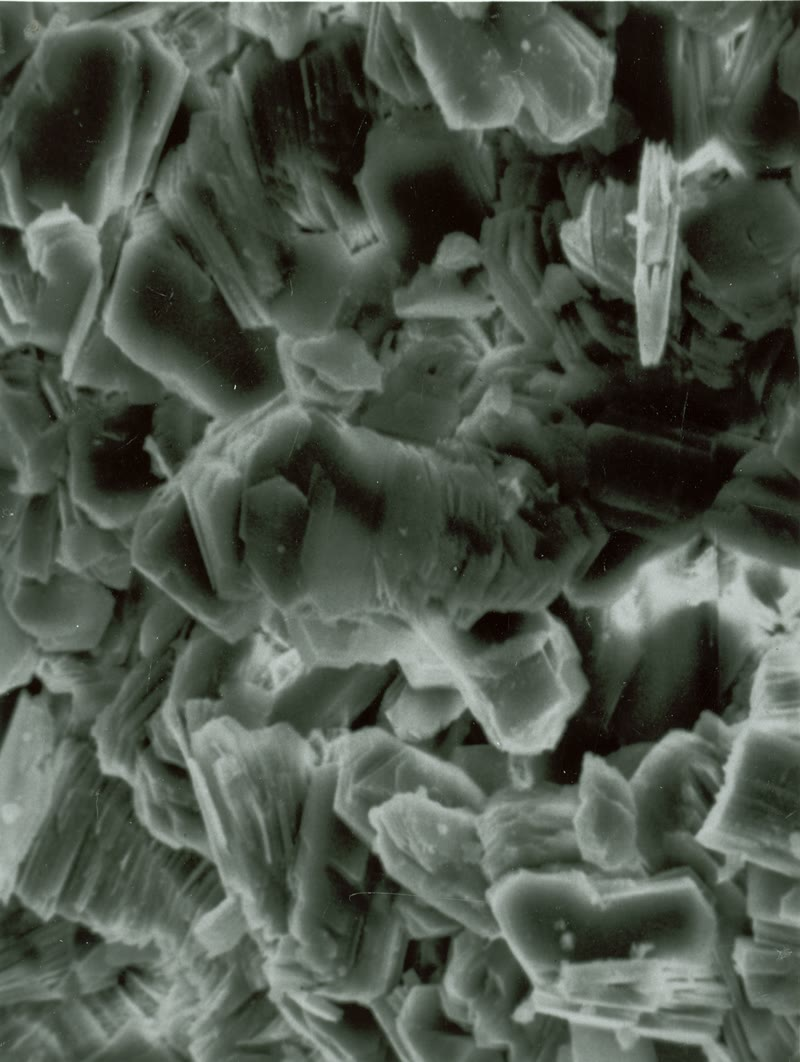
\includegraphics[width=\linewidth]{images/book3/b1-kaolinite-sem.jpg}

{\scriptsize \omterm{def:b1:weathering-clays:clay-mineral}{Caolinita} vista con un microscopio electrónico de barrido: libros de placas hexagonales apiladas, crecidas en los poros de una
arenisca del norte de Alaska (aumento de unas 1340 veces). Servicio Geológico de los Estados Unidos, dominio público, a través de
Wikimedia Commons.\par}
\end{minipage}
\end{omfigure}
% ledger: biscaye:1965, usgs:clay-settings, pedron:stages, commons:kaolinite-sem

\emph{\omterm{def:b1:weathering-clays:laterite}{Lateritas}.} Donde la \omterm{def:b1:weathering-clays:hydrolysis}{hidrólisis} alcanza sus últimos grados durante mucho tiempo, el perfil se engruesa y su parte superior concentra
todo lo que no sale.

\begin{definition}[Laterita]\label{def:b1:weathering-clays:laterite}
Una \emph{laterita}\index{laterita} es el producto, rico en hierro y aluminio, de una \omterm{def:b1:weathering-clays:hydrolysis}{hidrólisis} intensa y prolongada bajo climas cálidos y
húmedos: un material rojo a pardo, blando o endurecido, formado por \omterm{def:b1:weathering-clays:clay-mineral}{caolinita} y óxidos e hidróxidos de hierro, con gibbsita donde se llega a
la \omterm{def:b1:weathering-clays:hydrolysis-degree}{alitización}, del que han salido casi todos los cationes alcalinos y alcalinotérreos y gran parte de la sílice.
\end{definition}
% ledger: formoso:laterite, buchanan:laterite

Una \omterm{def:b1:weathering-clays:laterite}{laterita} lo bastante rica en gibbsita o en boehmita, los hidróxidos de aluminio, es una bauxita, el \omterm{def:b1:rock-forming-minerals:mineral}{mineral} de nueve décimas partes del
aluminio: la \omterm{def:b1:weathering-clays:hydrolysis-degree}{alitización} es el paso que hace el \omterm{def:b1:rock-forming-minerals:mineral}{mineral}. La mayoría de las bauxitas son residuales, la roca de la que se ha lixiviado todo menos
la alúmina; la mayoría de las formadas por gibbsita se encuentran en los trópicos, y muchas probablemente se están formando todavía.
% ledger: usgs:bauxite

\begin{history}[Una palabra del campo]
En 1807 Francis Buchanan, viajando por Malabar, en el sur de la India, describió un material lleno de cavidades y rico en ocres rojos y
amarillos de hierro, extendido sobre el granito en grandes masas. Extraído del suelo era tan blando que lo cortaba un cuchillo, y los habitantes
le daban forma de bloques; al aire pronto se volvía tan duro como el ladrillo, y duraba mejor que cualquier ladrillo que él hubiera visto. Las
lenguas locales lo llamaban piedra-ladrillo; él propuso el nombre de \omterm{def:b1:weathering-clays:laterite}{laterita}, que la geología conservó para los productos rojos de la
meteorización tropical.
\end{history}
% ledger: buchanan:laterite

\section{Meteorización de silicatos y dióxido de carbono}\label{sec:b1:weathering-clays:co2}

Los iones hidrógeno de la \omterm{def:b1:weathering-clays:hydrolysis}{hidrólisis} proceden sobre todo del dióxido de carbono, así que escribirlos como ácido carbónico muestra lo que la
meteorización hace al aire. Para un silicato de calcio, escrito \ce{CaSiO3} por sencillez,
\[
  \ce{CaSiO3 + 2 CO2 + H2O -> Ca^2+ + 2 HCO3- + SiO2},
\]
y en el océano, donde los organismos construyen conchas de carbonato de calcio,
\[
  \ce{Ca^2+ + 2 HCO3- -> CaCO3 + CO2 + H2O}.
\]

\begin{proposition}[Meteorización y dióxido de carbono]\label{prop:b1:weathering-clays:co2}
(a) La meteorización de un silicato consume dos moles de dióxido de carbono, convertidos en bicarbonato, por cada mol de calcio o de magnesio
liberado; cuando el calcio o el magnesio se precipitan como carbonato, uno de los dos vuelve al aire, y un mol queda almacenado como roca carbonatada.
(b) La meteorización de una roca carbonatada y la reprecipitación de su carbonato no almacenan ninguno.
\end{proposition}

\begin{proof}
(a) Sumando las dos ecuaciones anteriores resulta \ce{CaSiO3 + CO2 -> CaCO3 + SiO2}:
un \ce{CO2} por calcio sale del aire para siempre; la primera ecuación sola muestra los dos consumidos. Para el magnesio vale lo mismo, con \ce{Mg^2+} en lugar de
\ce{Ca^2+}. (b) La disolución de la calcita, \ce{CaCO3 + CO2 + H2O -> Ca^2+ + 2
HCO3-}, es exactamente lo contrario de la precipitación: la suma de las dos es cero.
\end{proof}

Con un \omterm{def:b1:rock-forming-minerals:groups}{feldespato}, el ácido carbónico sustituye a los iones hidrógeno de
\cref{prop:b1:weathering-clays:feldspars}: cada \ce{H+} consumido es un \ce{CO2} convertido en \ce{HCO3-}. La anortita de un basalto o de un gabro
consume así dos moles de dióxido de carbono por mol al convertirse en \omterm{def:b1:weathering-clays:clay-mineral}{caolinita},
\[
  \ce{CaAl2Si2O8 + 2 CO2 + 3 H2O -> Al2Si2O5(OH)4 + Ca^2+ + 2 HCO3-},
\]
y almacena uno a largo plazo. El sodio y el potasio no forman carbonato en el fondo marino, y el almacenamiento a largo plazo se cuenta a partir del
calcio y del magnesio liberados.

Los ríos llevan el bicarbonato al mar, y su química mide el flujo. A partir de la química de los grandes ríos del mundo se ha estimado que el dióxido
de carbono consumido por la meteorización de los silicatos continentales está entre \num{11.7e12} y \qty{13.6e12}{mol} al año, unos 0.14 a 0.16 mil millones de
toneladas de carbono, de las que la meteorización de los basaltos explica por sí sola entre el 30 y el \qty{35}{\percent}. El flujo es pequeño frente
a los intercambios de carbono entre el aire, los océanos y los seres vivos, pero no se invierte: a lo largo de millones de años es la vía principal por la que
el dióxido de carbono aportado por los volcanes sale de la atmósfera. Como la meteorización se acelera cuando hace más calor y más humedad, liga el dióxido
de carbono del aire al clima, que a su vez depende del dióxido de carbono a través del efecto invernadero: una retroalimentación negativa que estabiliza la
temperatura de la Tierra a lo largo del tiempo geológico, estudiada en el volumen del año~2.
% ledger: dessert:silicate-co2, whk:1981

\section{Ejercicios}

\begin{exercise}[$\star$]\label{exo:b1:weathering-clays:1}
Con los radios \ce{K+} \qty{1.38}{\angstrom}, \ce{Fe^2+} \qty{0.78}{\angstrom}, \ce{Fe^3+} \qty{0.645}{\angstrom} y \ce{Ti^4+} \qty{0.605}{\angstrom},
calcúlese el \omterm{def:b1:weathering-clays:ionic-potential}{potencial iónico} de cada ion y dígase su campo. ¿Por qué un suelo encharcado pierde su hierro mientras que uno bien drenado lo conserva?
% ledger: shannon:radii-b19
\end{exercise}

\begin{exercise}[$\star$]\label{exo:b1:weathering-clays:2}
Se radiografían cuatro fracciones de arcilla como preparaciones orientadas. A: un pico a
\SI{14}{\angstrom}, que pasa a \SI{17}{\angstrom} con etilenglicol y a \SI{10}{\angstrom} al calentar a \SI{400}{\celsius}. B: un pico a
\SI{7}{\angstrom}, sin cambio con glicol, que desaparece tras calentar a \SI{550}{\celsius}. C: un pico a \SI{10}{\angstrom} que ningún tratamiento
mueve. D: un pico a \SI{14}{\angstrom} que ningún tratamiento mueve. Identifíquese cada \omterm{def:b1:rock-forming-minerals:mineral}{mineral}.
% ledger: usgs:clay-xrd
\end{exercise}

\begin{exercise}[$\star$]\label{exo:b1:weathering-clays:3}
Ajústese, con \cref{met:b1:weathering-clays:balance}, la \omterm{def:b1:weathering-clays:hydrolysis}{hidrólisis} de la ortoclasa \ce{KAlSi3O8} a \omterm{def:b1:weathering-clays:clay-mineral}{caolinita}. ¿Qué fracción de su potasio y de
su silicio sale en disolución?
\end{exercise}

\begin{exercise}[$\star$]\label{exo:b1:weathering-clays:4}
(a) ¿Qué volumen de hielo produce \qty{10}{cm^3} de agua a \qty{0}{\celsius}? (b) ¿Dentro de qué intervalo de temperatura el hielo que crece en las
grietas parte la roca con mayor eficacia, y por qué ni una helada más suave ni una más dura lo hacen igual de bien? (c) Un cubo de granito de lado
\qty{1}{m} es partido por la helada en cubos de lado \qty{1}{cm}: ¿por qué factor ha crecido su superficie?
% ledger: usgs:water-density, iapws:ice-density, wh85:frost
\end{exercise}

\begin{exercise}[$\star\star$]\label{exo:b1:weathering-clays:5}
Calcúlese la superficie específica de granos de \omterm{def:b1:rock-forming-minerals:groups}{feldespato} de densidad \qty{2600}{kg.m^{-3}}, tratados como cubos, para tamaños de \qty{1}{cm},
\qty{1}{mm} y \qty{1}{\micro m}. ¿Por qué el tamaño del grano importa tanto para la velocidad de la \omterm{def:b1:weathering-clays:weathering}{meteorización química}, y por qué la \omterm{def:b1:weathering-clays:weathering}{meteorización
física} acelera la \omterm{def:b1:weathering-clays:weathering}{meteorización química}?
\end{exercise}

\begin{exercise}[$\star\star$]\label{exo:b1:weathering-clays:6}
Una tonelada de albita \ce{NaAlSi3O8} (\qty{262.22}{g.mol^{-1}}) se convierte en \omterm{def:b1:weathering-clays:clay-mineral}{caolinita} (\qty{258.16}{g.mol^{-1}}). Calcúlense la masa de \omterm{def:b1:weathering-clays:clay-mineral}{caolinita}
formada, la masa de sílice exportada, contada como \ce{SiO2} (\qty{60.08}{g.mol^{-1}}), y la masa de sodio exportada.
% ledger: webmineral:clays-b19, ciaaw:Na
\end{exercise}

\begin{exercise}[$\star\star$]\label{exo:b1:weathering-clays:7}
Un granito contiene, en masa, \qty{0.30}{\percent} de \ce{TiO2}, \qty{3.5}{\percent}
de \ce{Na2O}, \qty{72}{\percent} de \ce{SiO2} y \qty{14}{\percent} de \ce{Al2O3}; su saprolita
contiene \qty{0.60}{\percent} de \ce{TiO2}, \qty{0.35}{\percent}
de \ce{Na2O}, \qty{60}{\percent} de \ce{SiO2} y \qty{27}{\percent} de \ce{Al2O3}.
Tomando el titanio como inmóvil, calcúlese la masa de saprolita que deja un kilogramo de
granito, y la fracción de sodio, de silicio y de aluminio perdida. ¿Qué grado de
\omterm{def:b1:weathering-clays:hydrolysis}{hidrólisis} está en marcha?
\end{exercise}

\begin{exercise}[$\star\star$]\label{exo:b1:weathering-clays:8}
Con \cref{prop:b1:weathering-clays:layer-charge}, calcúlese la carga de la capa de
pirofilita \ce{Al2Si4O10(OH)2}, de la moscovita \ce{KAl2(Si3Al)O10(OH)2} sin su potasio, de la capa de
beidellita \ce{Al2(Si_{3.5}Al_{0.5})O10(OH)2} y de una capa de montmorillonita
\ce{(Al_{1.67}Mg_{0.33})Si4O10(OH)2}. ¿Cuáles de ellas pueden hincharse, y por qué?
% ledger: webmineral:clays-b19
\end{exercise}

\begin{exercise}[$\star\star$]\label{exo:b1:weathering-clays:9}
\ce{Mg2SiO4} (forsterita) se meteoriza según
\ce{Mg2SiO4 + 4 CO2 + 4 H2O -> 2 Mg^2+ + 4 HCO3- + H4SiO4}. (a) Compruébese la
ecuación. (b) Para una tonelada de forsterita, calcúlese el dióxido de carbono consumido y el
dióxido de carbono almacenado a largo plazo según
\cref{prop:b1:weathering-clays:co2}. (c) ¿Qué daría el mismo cálculo para una tonelada de calcita?
% ledger: ciaaw:Mg, ciaaw:Si, ciaaw:O, ciaaw:C
\end{exercise}

\begin{exercise}[$\star\star\star$]\label{exo:b1:weathering-clays:10}
(a) ¿Entre qué radios es hidrolizado un ion de carga 3? (b) El boro, \ce{B^3+}, tiene un radio de
\qty{0.27}{\angstrom}: ¿en qué forma viaja en el agua? (c) \ce{Mn^2+} tiene un radio de
\qty{0.83}{\angstrom}, \ce{Mn^4+} de \qty{0.53}{\angstrom}. Explíquese por qué se forman costras negras de óxido de manganeso donde el agua de
manantial, pobre en oxígeno, sale al aire. (d) ¿Por qué el silicio no puede ser ni lixiviado por completo ni conservado por completo?
% ledger: shannon:radii-b19, nomad:goldschmidt
\end{exercise}

\begin{exercise}[$\star\star\star$]\label{exo:b1:weathering-clays:11}
La meteorización de los silicatos continentales consume entre \num{11.7e12} y
\qty{13.6e12}{mol} de dióxido de carbono al año, de ellos \qty{4.08e12}{mol} procedentes de
basaltos. (a) Conviértase el intervalo en toneladas de carbono y de dióxido de carbono al año. (b) ¿Qué fracción corresponde a los basaltos?
(c) Si todo esto procediera de silicatos de calcio y de magnesio, ¿cuánto carbono se almacenaría a largo plazo cada año? ¿Por qué la cifra real a
largo plazo es menor?
% ledger: dessert:silicate-co2, ciaaw:C, ciaaw:O
\end{exercise}

\begin{exercise}[$\star\star\star$]\label{exo:b1:weathering-clays:12}
Tres fracciones de arcilla, libres de cuarzo y de óxidos de hierro, se analizan (porcentaje en masa): A, \ce{SiO2} \num{46.55} y \ce{Al2O3} \num{39.50};
B, \ce{SiO2} 60 y \ce{Al2O3} 25; C, \ce{SiO2} 2 y \ce{Al2O3} 63 (\ce{SiO2}
\qty{60.08}{g.mol^{-1}}, \ce{Al2O3} \qty{101.96}{g.mol^{-1}}). Calcúlese el cociente molar Si/Al de cada una, identifíquese el grado de
\omterm{def:b1:weathering-clays:hydrolysis}{hidrólisis} que registra, y colóquense los tres suelos en una recta, desde la lixiviación menos intensa hasta la más intensa.
% ledger: webmineral:clays-b19, pedron:stages, formoso:laterite
\end{exercise}

\section{Problema: del granito a la arcilla}

\begin{problem}[{Problema de fin de semana --- los feldespatos de un granito y de un gabro, desde las reacciones ajustadas hasta el dióxido de
carbono que se lleva un río}]
\label{pb:b1:weathering-clays:1}
% values: calc/ch19.py; the river is invented (its numbers are of a realistic order)
Los \omterm{def:b1:rock-forming-minerals:groups}{feldespatos} son la albita \ce{NaAlSi3O8} (\qty{262.22}{g.mol^{-1}}, densidad
\qty{2.62}{g.cm^{-3}}) y la anortita \ce{CaAl2Si2O8}
(\qty{278.20}{g.mol^{-1}}, densidad \qty{2.75}{g.cm^{-3}}). La \omterm{def:b1:weathering-clays:clay-mineral}{caolinita}
\ce{Al2Si2O5(OH)4} tiene la masa molar \qty{258.16}{g.mol^{-1}} y la densidad
\qty{2.6}{g.cm^{-3}}; la gibbsita \ce{Al(OH)3}, \qty{78.00}{g.mol^{-1}}. Tómense
\ce{SiO2} \qty{60.08}{g.mol^{-1}}, \ce{CO2} \qty{44.01}{g.mol^{-1}}, \ce{HCO3-}
\qty{61.02}{g.mol^{-1}}, Na \num{22.99} y Ca \qty{40.08}{g.mol^{-1}}.
% ledger: hom:albite, hom:anorthite, webmineral:clays-b19, ciaaw:Na, ciaaw:Ca, ciaaw:C, ciaaw:O, ciaaw:H

\medskip
\noindent\textbf{Parte I --- Las reacciones.}
\begin{enumerate}
  \item Ajústese la \omterm{def:b1:weathering-clays:hydrolysis}{hidrólisis} de la albita a \omterm{def:b1:weathering-clays:clay-mineral}{caolinita}.
  \item Ajústese la \omterm{def:b1:weathering-clays:hydrolysis}{hidrólisis} de la anortita a \omterm{def:b1:weathering-clays:clay-mineral}{caolinita}. ¿Qué tiene de especial?
  \item Ajústese la \omterm{def:b1:weathering-clays:hydrolysis}{hidrólisis} de la anortita a gibbsita.
  \item Ajústese la \omterm{def:b1:weathering-clays:hydrolysis}{hidrólisis} de la albita a beidellita
        \ce{Na_{0.5}Al2(Si_{3.5}Al_{0.5})O10(OH)2}, y compruébese el hidrógeno.
  \item Reescríbanse las dos primeras reacciones con el ácido carbónico como fuente de
        los iones hidrógeno: \ce{CO2 + H2O -> H+ + HCO3-}.
  \item ¿Cuáles de estas reacciones son \omterm{def:b1:weathering-clays:hydrolysis-degree}{bisialitización}, \omterm{def:b1:weathering-clays:hydrolysis-degree}{monosialitización} y \omterm{def:b1:weathering-clays:hydrolysis-degree}{alitización}?
\end{enumerate}

\medskip
\noindent\textbf{Parte II --- Qué queda y qué sale.}
\begin{enumerate}[resume]
  \item ¿Cuántos moles hay en una tonelada de albita, y en una tonelada de anortita?
  \item Calcúlese la masa de \omterm{def:b1:weathering-clays:clay-mineral}{caolinita} formada a partir de una tonelada de cada una.
  \item Calcúlense las masas de sílice (como \ce{SiO2}), de sodio y de calcio exportadas en disolución.
  \item Calcúlese el volumen de una tonelada de cada \omterm{def:b1:rock-forming-minerals:groups}{feldespato} y de la \omterm{def:b1:weathering-clays:clay-mineral}{caolinita} que da. ¿En qué fracción se contrae el volumen del sólido?
  \item Una saprolita conserva la forma de la roca que reemplaza. ¿Qué llena el espacio que queda en un granito meteorizado rico en albita?
        ¿Por qué un gabro meteorizado rico en anortita sigue siendo más denso?
  \item Con el diagrama del \omterm{def:b1:weathering-clays:ionic-potential}{potencial iónico}, explíquese qué elementos de los dos \omterm{def:b1:rock-forming-minerals:groups}{feldespatos} salen y cuáles quedan.
\end{enumerate}

\medskip
\noindent\textbf{Parte III --- Dióxido de carbono.}
\begin{enumerate}[resume]
  \item ¿Cuántos moles, y cuántos kilogramos, de dióxido de carbono se consumen cuando una tonelada de albita se convierte en \omterm{def:b1:weathering-clays:clay-mineral}{caolinita}?
  \item La misma pregunta para una tonelada de anortita.
  \item ¿Qué masa de bicarbonato exporta la anortita?
  \item ¿Qué le ocurre a este bicarbonato en el océano? ¿Cuánto del dióxido de carbono consumido vuelve al aire?
  \item ¿Por qué no se cuenta almacenamiento a largo plazo para el sodio de la albita?
  \item Compárese con la disolución de una tonelada de calcita seguida de su precipitación.
\end{enumerate}

\medskip
\noindent\textbf{Parte IV --- Un río.}
\begin{enumerate}[resume]
  \item Un río drena \qty{50000}{km^2} de granito y gneis, con un caudal medio de \qty{200}{m^3.s^{-1}}; el bicarbonato que lleva de la
        meteorización de silicatos es \qty{0.3}{mmol.L^{-1}}. Calcúlese el flujo anual de este bicarbonato, en moles, y por kilómetro cuadrado.
  \item Exprésese como los moles de anortita cuya meteorización a \omterm{def:b1:weathering-clays:clay-mineral}{caolinita} lo suministraría, y después como toneladas de anortita al año y
        por kilómetro cuadrado.
  \item Si la roca contiene el equivalente de un \qty{20}{\percent} de anortita y tiene la densidad \qty{2700}{kg.m^{-3}}, ¿a qué velocidad, en
        metros por millón de años, se consume la roca fresca?
  \item ¿Cuánto dióxido de carbono quita este río del aire, para siempre, cada año?
  \item ¿Por qué la velocidad de la pregunta 21 es una cota inferior del descenso de la superficie del terreno?
  \item En kilogramos, con tres cifras, ¿cuánto dióxido de carbono se retira para siempre por la meteorización de una tonelada de anortita?
\end{enumerate}
\end{problem}
